\section{Dữ liệu 2: Hồi quy thành phần chính}

\subsection*{Giới thiệu bộ dữ liệu}
Hiện nay, Xe đạp cho thuê được giới thiệu ở nhiều thành phố để nâng cao sự thoải mái khi di chuyển. Điều cần quan tâm khi cho thuê xe đạp là xe đạp phải luôn sẵn sàng và tiếp cận được người dùng vào đúng thời điểm, giúp giảm bớt thời gian chờ. Do đó, việc đảm bảo một nguồn cung cấp xe đạp cho thuê ổn định cho thành phố trở thành mối quan tâm lớn. Phần quan trọng là cần dự đoán được số lượng xe đạp cần thiết tại mỗi giờ, để có được nguồn cung cấp xe đạp cho thuê ổn định.

Nhóm em sử dụng bộ dữ liệu Nhu cầu thuê xe đạp ở Seoul\footnote{\url{https://archive.ics.uci.edu/ml/datasets/Seoul+Bike+Sharing+Demand}} (\textbf{Seoul Bike Sharing Demand Dataset}).

Bộ dữ liệu ghi lại các thông tin về thời tiết, số lượng xe đạp được thuê mỗi giờ theo từng ngày, từ 01/12/2017 đến 31/11/2018. Bộ dữ liệu có 8760 quan trắc, gồm 14 biến sau:
\begin{enumerate}
	\item \textbf{Date} - Ngày ghi lại số lượng xe đạp cho thuê
	\item \textbf{Rented Bike count} - Số lượng xe đạp được thuê được ghi lại theo mỗi giờ
	\item \textbf{Hour} - Giờ trong ngày
	\item \textbf{Temperature} - Nhiệt độ ($^o C$)
	\item \textbf{Humidity} - Độ ẩm (\%)
	\item \textbf{Windspeed} - Tốc độ gió ($m/s$)
	\item \textbf{Visibility} - Tầm nhìn xa ($10m$)
	\item \textbf{Dew point temperature} - Nhiệt độ điểm sương ($^o C$)
	\item \textbf{Solar radiation} - Bức xạ mặt trời ($Mj/m^2$)
	\item \textbf{Rainfall} - Lượng mưa ($mm$)
	\item \textbf{Snowfall} - Lượng tuyết rơi ($cm$)
	\item \textbf{Seasons} - Mùa (Winter, Spring, Summer, Autumn)
	\item \textbf{Holiday} - Ngày lễ (Holiday/No holiday)
	\item \textbf{Functional Day} - Ngày làm việc (Yes nếu là ngày làm việc, No nếu ngược lại)
\end{enumerate}

Một vài quan trắc đầu tiên trong bộ dữ liệu được thể hiện trong hình \ref{A2_head}

\begin{figure}[H]
	\centering
	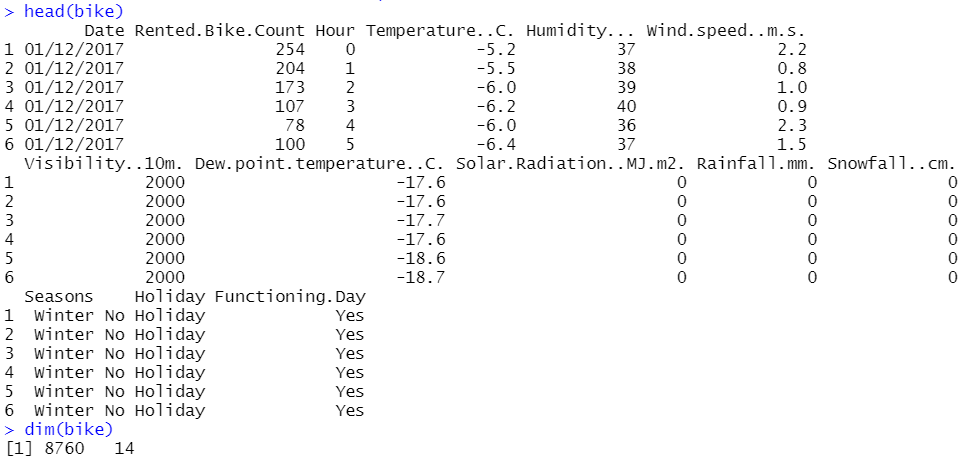
\includegraphics[width=0.8\linewidth]{../Photo Of Result/A2_head}
	\caption{Một vài quan trắc đầu tiên và số chiều của bộ dữ liệu}
	\label{A2_head}
\end{figure}

\subsection*{Phân tích và chọn mô hình}

\begin{figure}[H]
	\centering
	\subfloat[...]
	{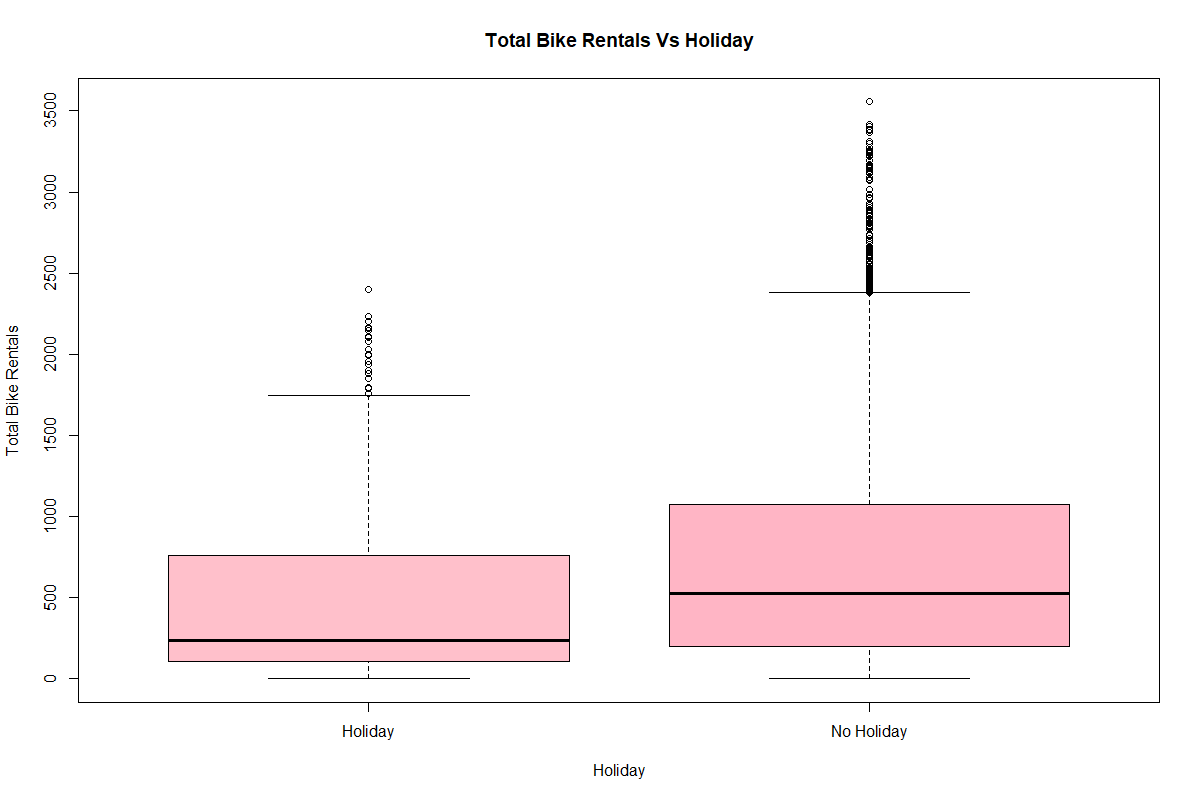
\includegraphics[width=.5\linewidth]{../Photo Of Result/A2_boxplot1}}\hfill
	\subfloat[Kiểm tra đa cộng tuyến]
	{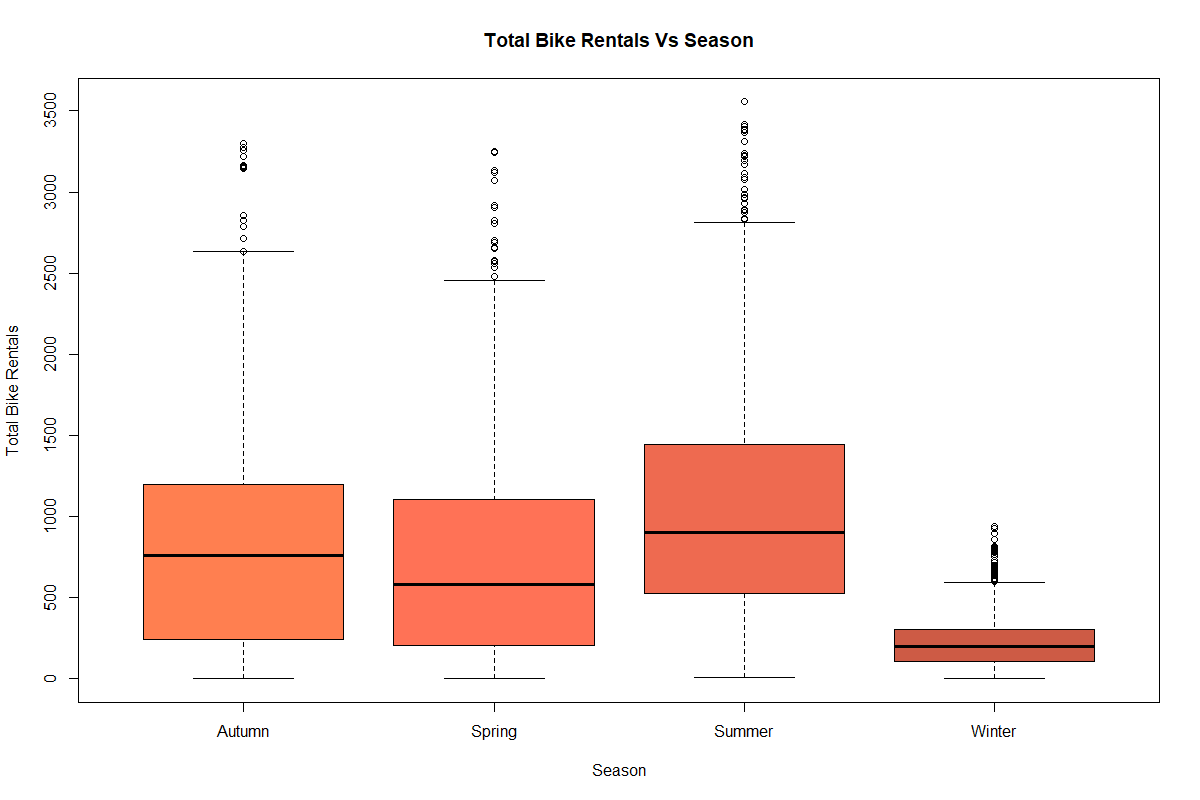
\includegraphics[width=.5\linewidth]{../Photo Of Result/A2_boxplot2}}\\
	\subfloat[...]
	{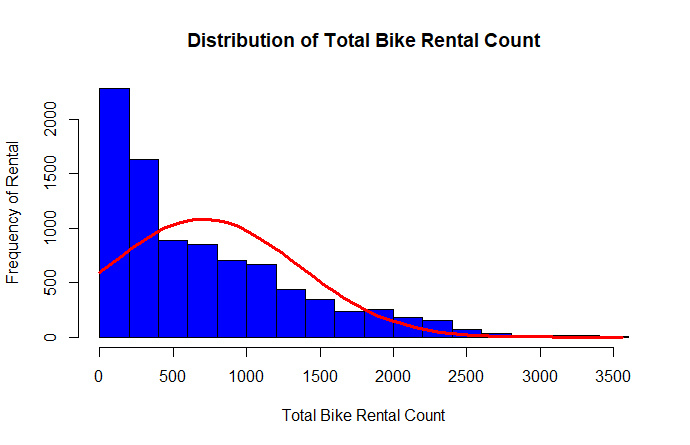
\includegraphics[width=.5\linewidth]{../Photo Of Result/A2_plotcount}}\hfill
	\subfloat[Kiểm tra đa cộng tuyến]
	{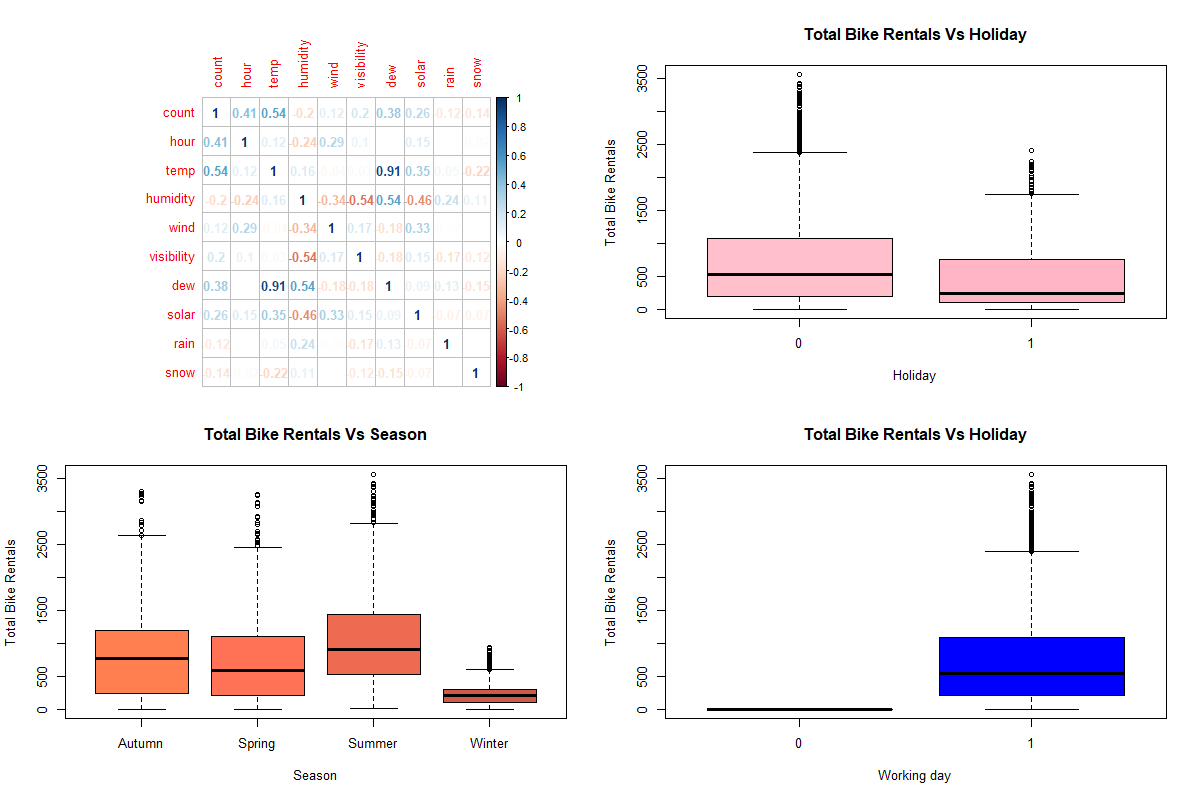
\includegraphics[width=.5\linewidth]{../Photo Of Result/A2_corr}}
	\caption{Một vài quan sát ...}
	\label{A2_visual}
\end{figure}

\begin{figure}[H]
	\centering
	\subfloat[...]
	{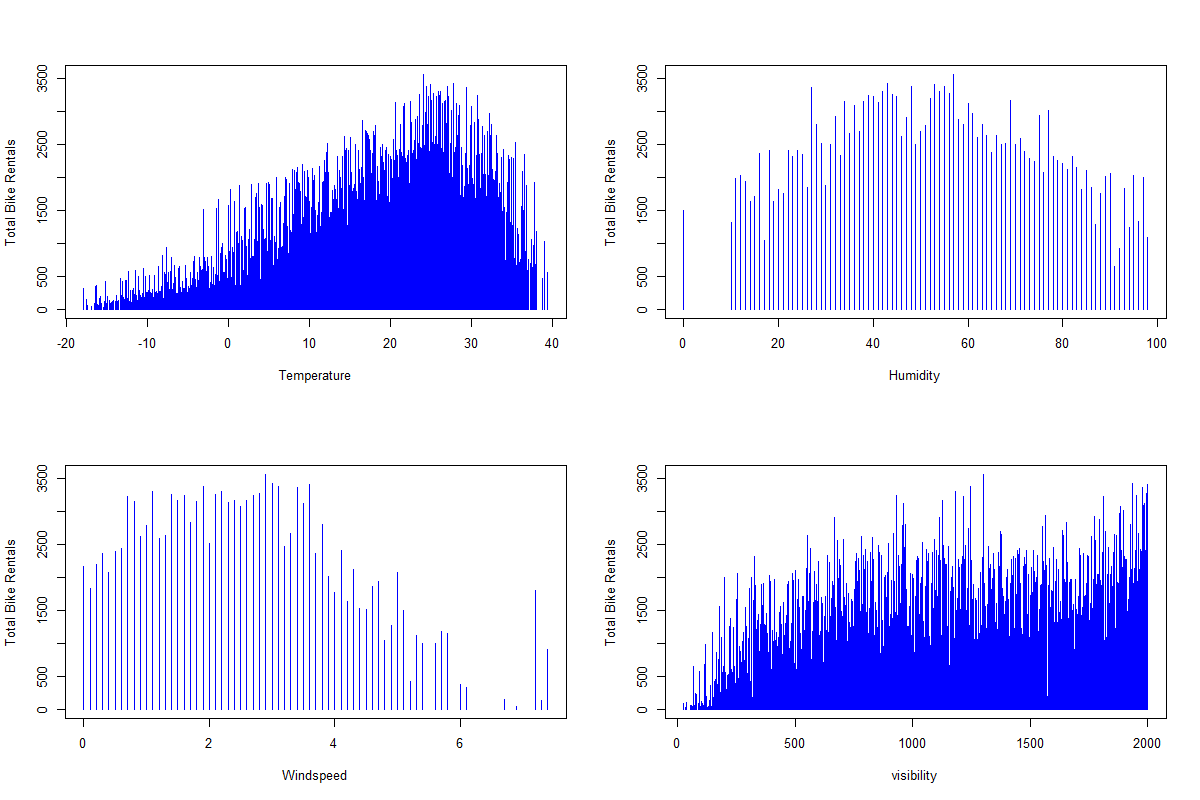
\includegraphics[width=.7\linewidth]{../Photo Of Result/A2_plotvar1}}\\
	\subfloat[Kiểm tra đa cộng tuyến]
	{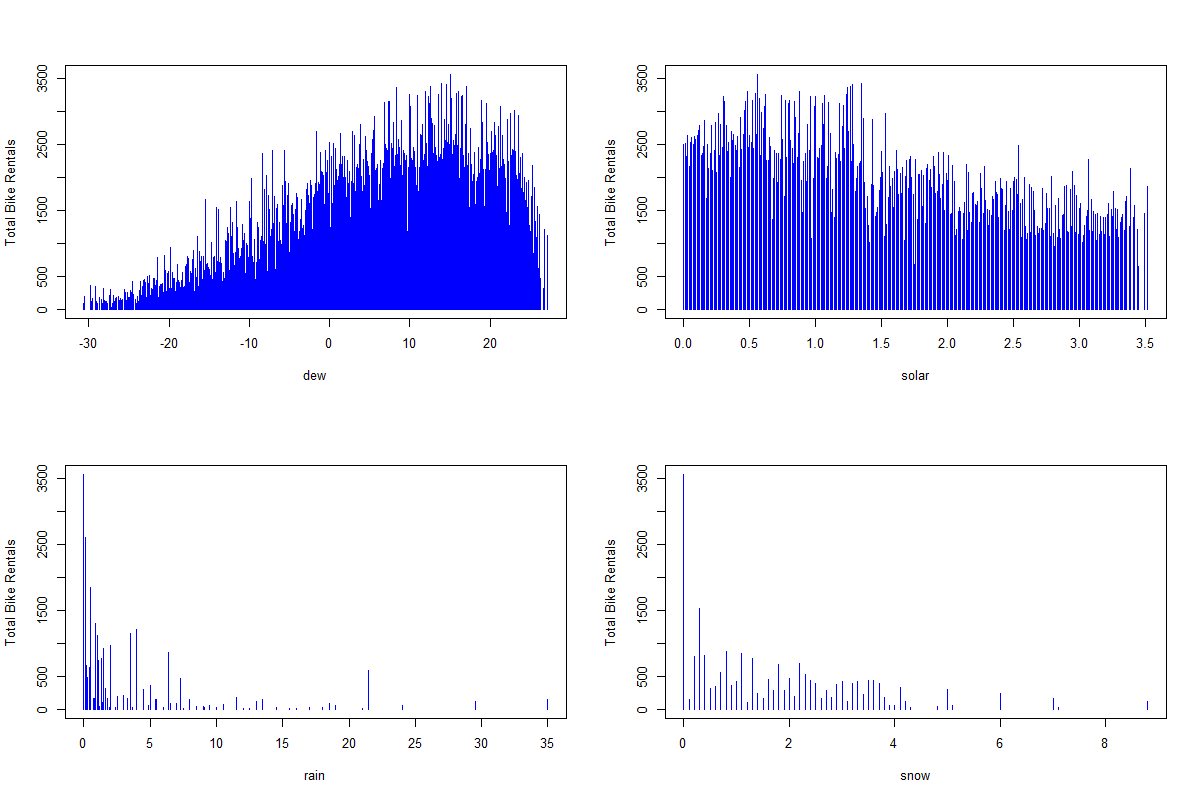
\includegraphics[width=.7\linewidth]{../Photo Of Result/A2_plotvar2}}
	\caption{Một vài quan sát ...}
	\label{A2_visual2}
\end{figure}

\subsection*{Nhận xét và kết luận}